\documentclass[11pt,a4paper]{article}
\usepackage[T1]{fontenc}
\usepackage[utf8]{inputenc}
\usepackage[polish]{babel}
\usepackage{lmodern,amsmath,amssymb,graphicx,booktabs}
\usepackage[margin=2.3cm]{geometry}
\usepackage[hidelinks]{hyperref}
\setlength{\parindent}{0pt}
\setlength{\parskip}{5pt}
\title{Metody identyfikacji - projekt 1\\[4pt]\large Usuwanie zakłóceń impulsowych z nagrań muzycznych}
\author{Paweł Dolak, 193582 \and Nikodem Bąk, 193338}
\date{}
\begin{document}
\maketitle

\section{Cel i dane}
Usuwanie trzasków metodą AR(4), EW-LS/RLS i interpolacji liniowej.

Zbadano pięć losowych nagrań, pierwszy kanał, $f_s=22050$ Hz. Oznaczenia: $x$ - wejście, $y$ - wynik. Nastawy jednakowe dla wszystkich prób.

\section{Model AR(4) i estymacja parametrów}
Historia predykcji $z$, rząd modelu 4:
\begin{equation}
\varphi(k)=[z(k-1),z(k-2),z(k-3),z(k-4)]^T.
\end{equation}
Predykcja i błąd przed aktualizacją:
\begin{equation}
\hat{x}(k)=a^T(k-1)\varphi(k),\qquad e(k)=x(k)-\hat{x}(k).
\end{equation}
Podstawowe kryterium EW-LS
\begin{equation}
J_k(a)=\sum_{i=4}^{k}\lambda^{k-i}\bigl[x(i)-a^T\varphi(i)\bigr]^2,
\end{equation}
Dla próbki zaakceptowanej:
\begin{align}
g(k)&=\frac{P(k-1)\varphi(k)}{\lambda+\varphi^T(k)P(k-1)\varphi(k)},\\
a(k)&=a(k-1)+g(k)e(k),\\
P(k)&=\frac{P(k-1)-g(k)\varphi^T(k)P(k-1)}{\lambda}.
\end{align}
Start: $a(3)=0$, $P(3)=1000I$. Dla próbki zakwestionowanej:
\begin{equation}
a(k)=a(k-1),\qquad P(k)=P(k-1)/\lambda.
\end{equation}


\subsection{Dwa warianty historii predykcji}
\textbf{A - z zakwestionowaną próbką:} $z_A(k)=x(k)$.

\textbf{B - z ostatnią zaakceptowaną próbką:}
\begin{equation}
z_B(k)=\begin{cases}
x(k), & \text{gdy próbka jest zaakceptowana},\\
z_B(k-1), & \text{gdy próbka jest zakwestionowana}.
\end{cases}
\end{equation}
Przed detekcją $z=x$. W obu wariantach końcową naprawą jest interpolacja; powtarzanie wartości w B dotyczy tylko historii modelu.



\section{Detekcja zakłóceń}
Okno $M$ wcześniejszych błędów, bez bieżącego:
\begin{align}
\bar e(k)&=\frac{1}{M}\sum_{i=k-M}^{k-1}e(i),\\
\sigma(k)&=\sqrt{\frac{1}{M}\sum_{i=k-M}^{k-1}\bigl[e(i)-\bar e(k)\bigr]^2}.
\end{align}
Próbka jest kwestionowana, gdy
\begin{equation}
|e(k)|>3\sigma(k).
\end{equation}
Pierwsze $M$ predykcji: rozruch bez detekcji. Wszystkie błędy, także zakwestionowanych próbek, uczestniczą w obliczaniu progu.

\section{Nastawy algorytmu}
\begin{center}
\begin{tabular}{lll}
\toprule
Parametr & Wartość & Znaczenie\\
\midrule
$\lambda$ & 0,999 & Współczynnik zapominania\\
$P(3)$ & $1000I$ & Inicjalizacja macierzy RLS\\
$M$ & 221 & Okno wcześniejszych błędów\\
\bottomrule
\end{tabular}
\end{center}
$\lambda=0{,}999$ daje wagę około $0{,}368$ dla obserwacji sprzed 1000 próbek (45 ms).

$M=221$ (10 ms) pozwala lokalnie dostosować próg. $P(3)=1000I$ umożliwia większe początkowe korekty. Nastawy nie są wynikiem optymalizacji.

\section{Rekonstrukcja próbek}
Dla serii $s,\ldots,u-1$, długości $L=u-s$:
\begin{equation}
y(s+j)=x(s-1)+\frac{j+1}{L+1}\bigl[x(u)-x(s-1)\bigr],\quad j=0,\ldots,L-1.
\end{equation}
Dla jednej próbki otrzymuje się
\begin{equation}
y(k)=\tfrac12\bigl[x(k-1)+x(k+1)\bigr].
\end{equation}
Naprawiane są serie 1-4 próbek z oboma sąsiadami. Dłuższe serie i serie na brzegu są pomijane.

\section{Porównanie wariantów A i B}
Te same pięć nagrań i nastawy dla A/B. Wyniki dotyczą całych plików.

Detekcje: zakwestionowane próbki. Rekonstrukcja: próbki interpolowane. RMSE zmiany:
\begin{equation}
D=\sqrt{\frac{1}{N}\sum_{k=0}^{N-1}[y(k)-x(k)]^2}.
\end{equation}
$D$ mierzy ingerencję w wejście, nie jakość odszumiania.

\begin{center}
\small
\setlength{\tabcolsep}{4pt}
\begin{tabular}{llrrrrr}
\toprule
Plik & Wariant & Detekcje & Rekonstr. & Udział [\%] & Pom. serie & $D$\\
\midrule
03.wav & A & 1663 & 1653 & 0,383 & 2 & 0,01192\\
03.wav & B & 11486 & 887 & 0,205 & 630 & 0,01186\\
04.wav & A & 1716 & 1711 & 0,406 & 1 & 0,01016\\
04.wav & B & 7586 & 1089 & 0,258 & 506 & 0,01025\\
17.wav & A & 3243 & 3191 & 1,467 & 9 & 0,01297\\
17.wav & B & 5642 & 1819 & 0,836 & 541 & 0,02247\\
22.wav & A & 1020 & 1020 & 0,449 & 0 & 0,01003\\
22.wav & B & 3178 & 743 & 0,327 & 226 & 0,01008\\
23.wav & A & 2120 & 2093 & 0,484 & 5 & 0,01756\\
23.wav & B & 3987 & 3170 & 0,734 & 112 & 0,02872\\
\bottomrule
\end{tabular}
\end{center}



Lewa kolumna: A, prawa: B. Wspólne skale. Parametry AR pokazano co dziesiątą próbkę; sygnały i błędy - w całości.

\clearpage
\subsection{Nagranie 03.wav}
\begin{figure}[htbp]
\centering
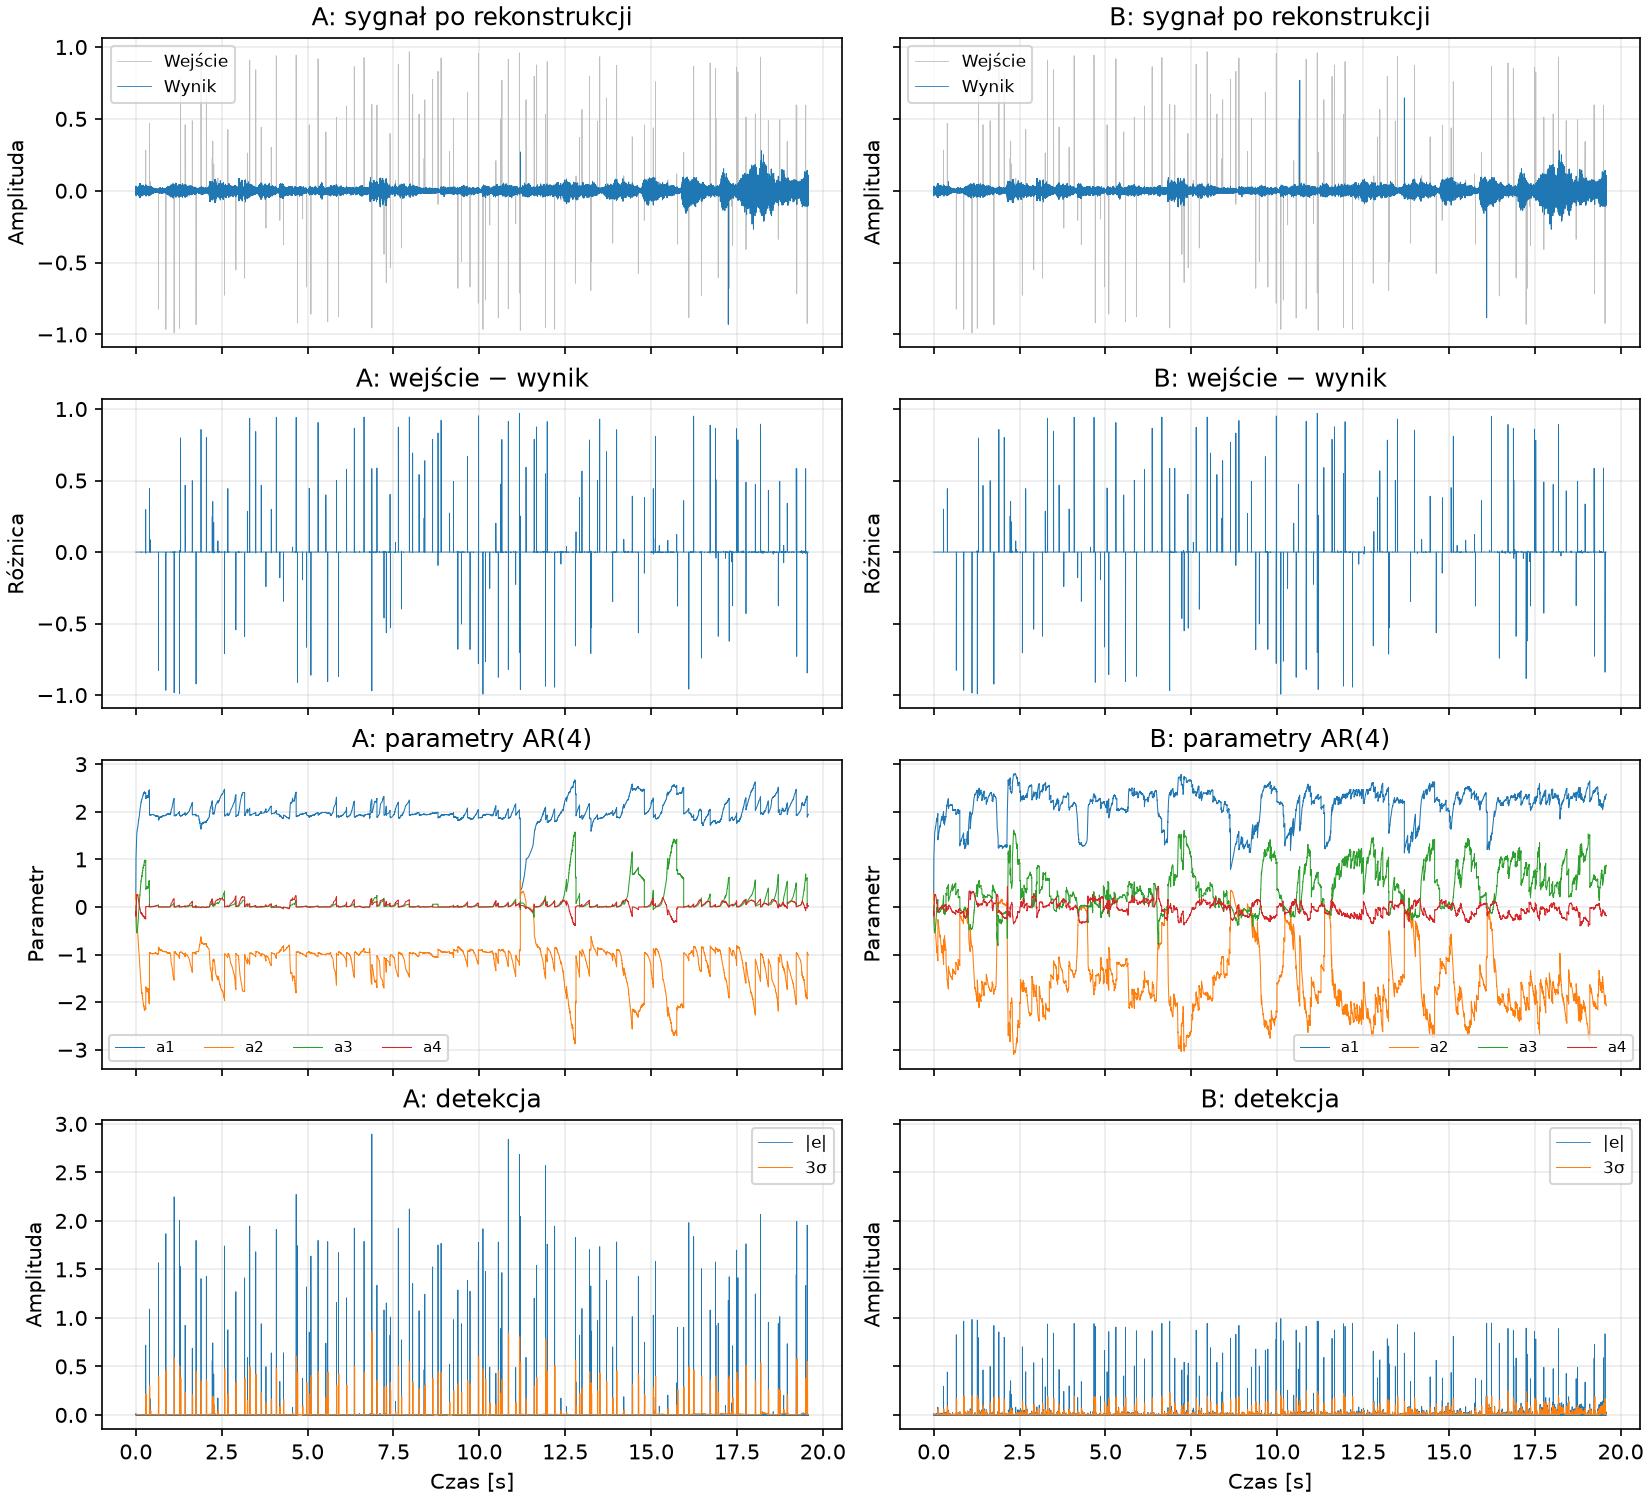
\includegraphics[width=\linewidth]{images/03_AB.png}
\caption{\texttt{03.wav}: A - z zakwestionowaną próbką, B - z ostatnią zaakceptowaną próbką.}
\end{figure}

\clearpage
\subsection{Nagranie 04.wav}
\begin{figure}[htbp]
\centering
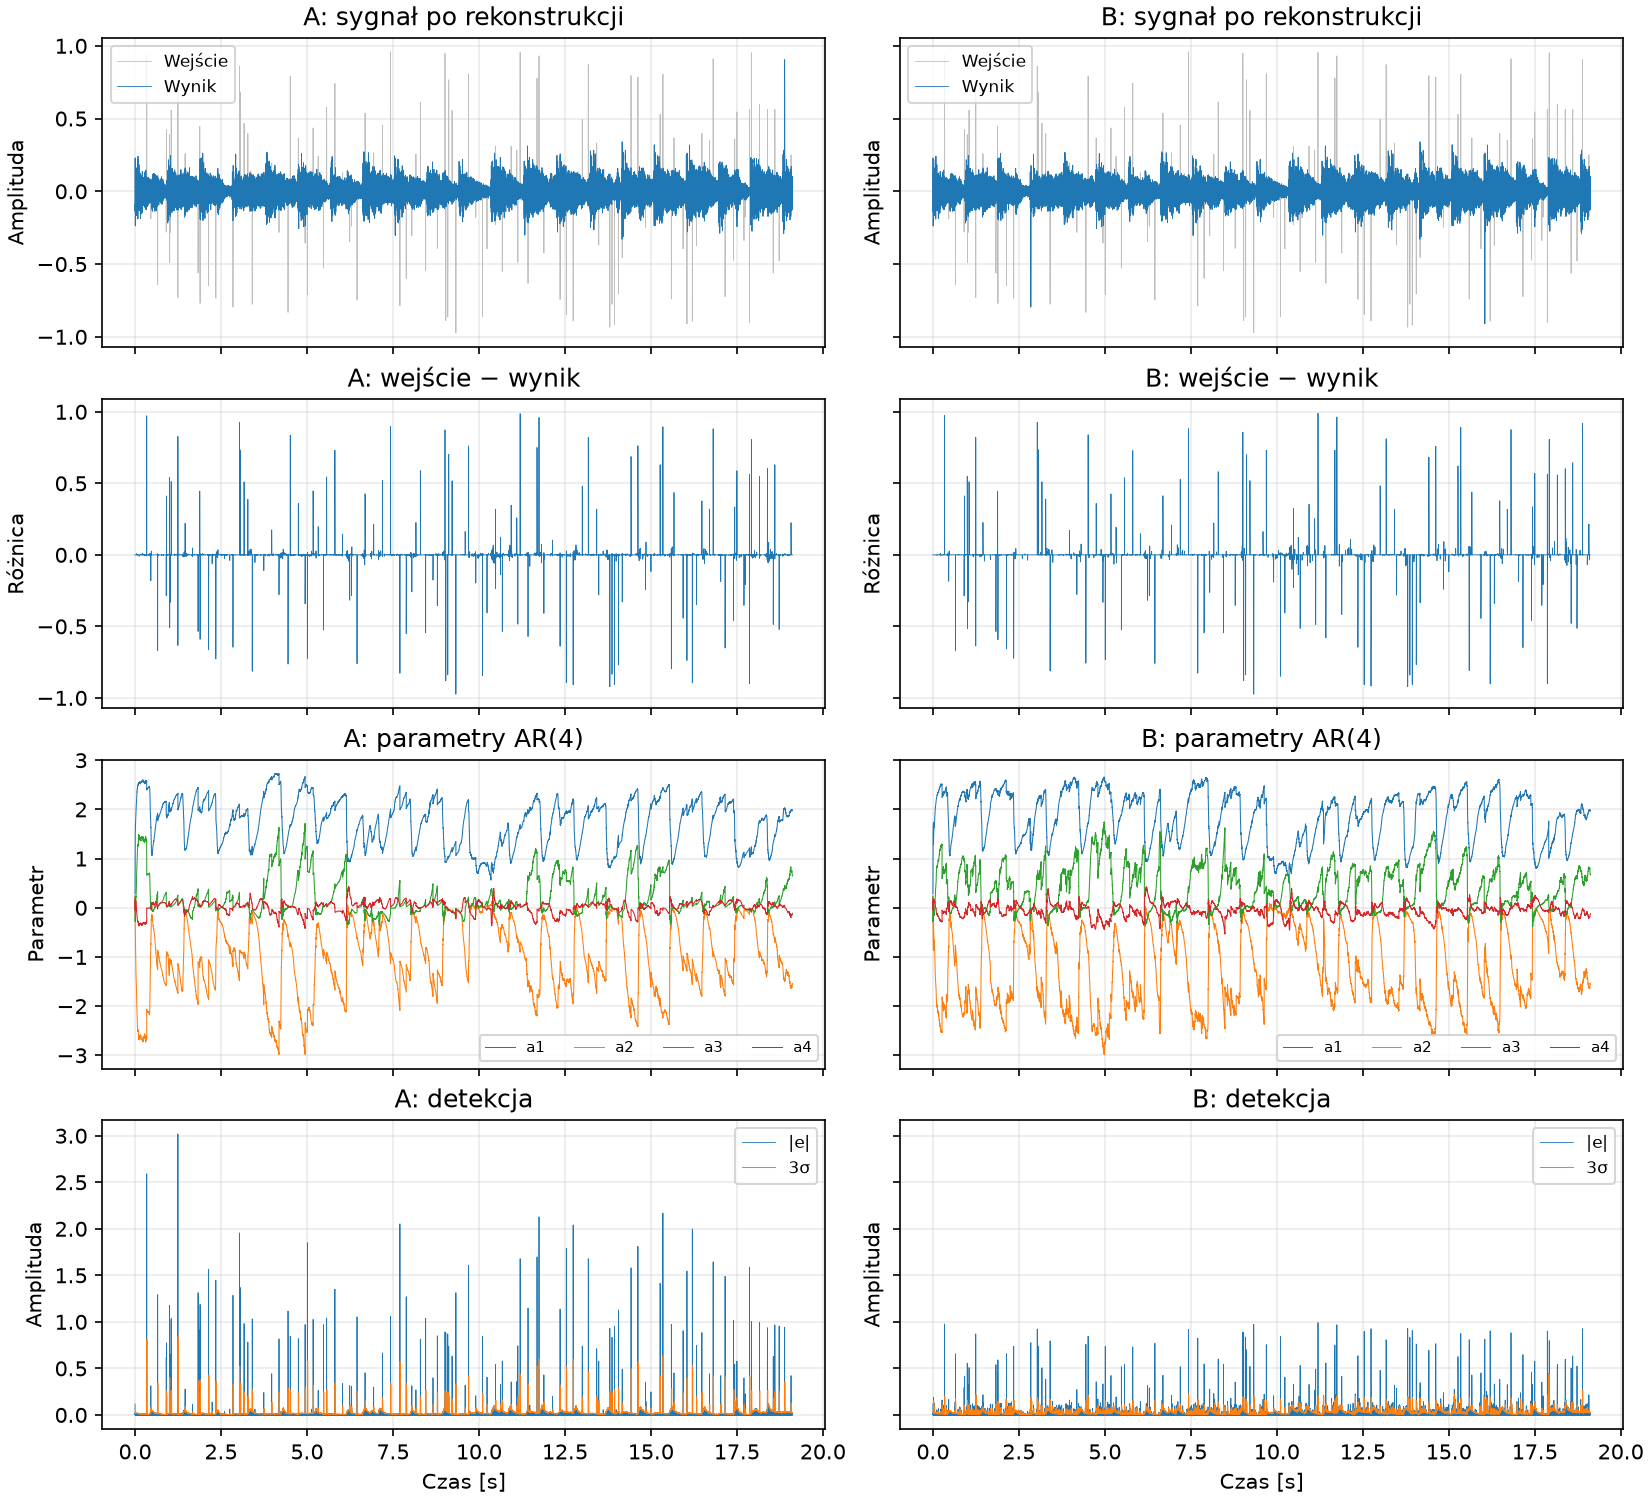
\includegraphics[width=\linewidth]{images/04_AB.png}
\caption{\texttt{04.wav}: A - z zakwestionowaną próbką, B - z ostatnią zaakceptowaną próbką.}
\end{figure}

\clearpage
\subsection{Nagranie 17.wav}
\begin{figure}[htbp]
\centering
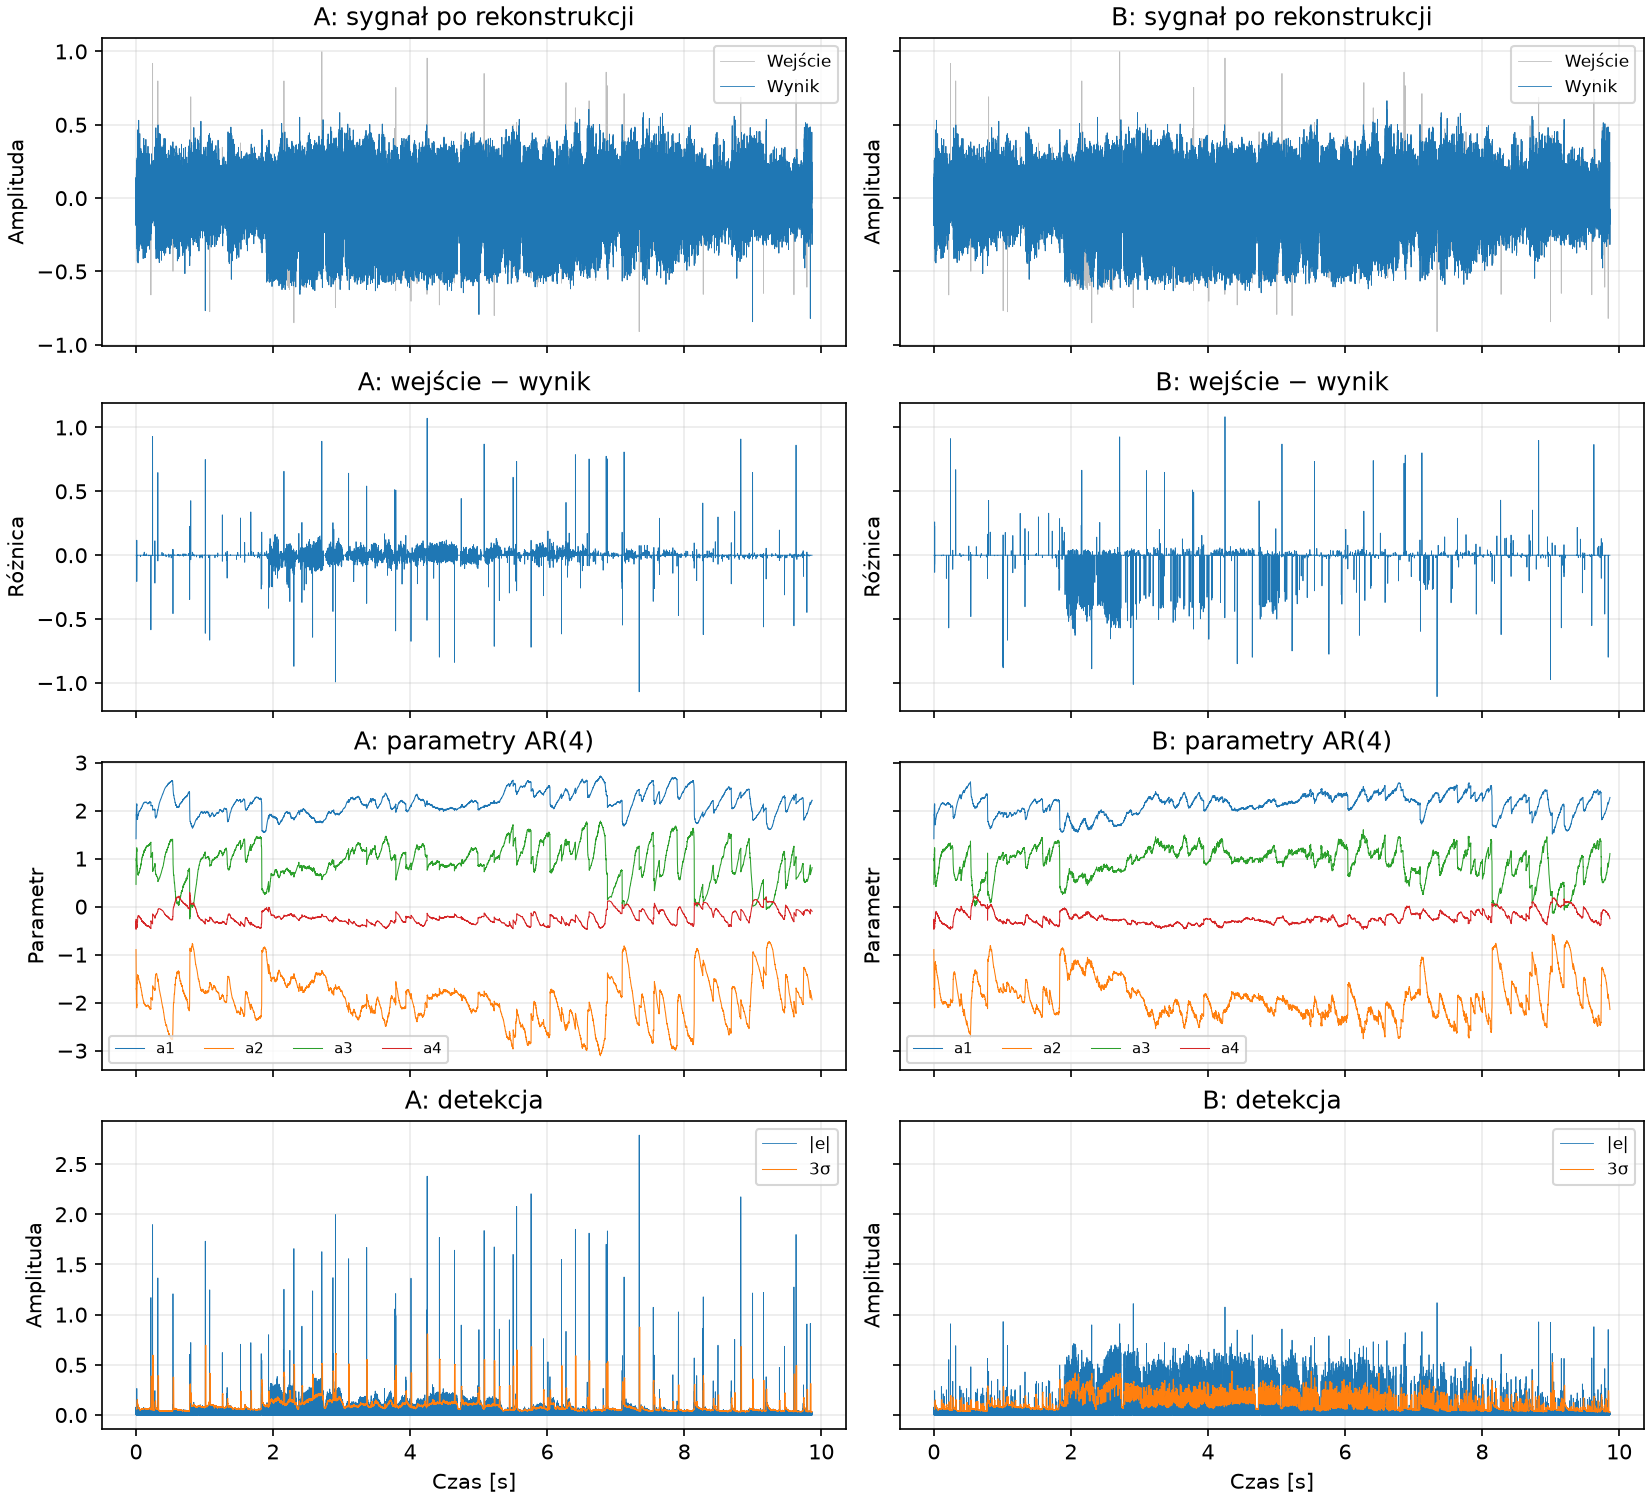
\includegraphics[width=\linewidth]{images/17_AB.png}
\caption{\texttt{17.wav}: A - z zakwestionowaną próbką, B - z ostatnią zaakceptowaną próbką.}
\end{figure}

\clearpage
\subsection{Nagranie 22.wav}
\begin{figure}[htbp]
\centering
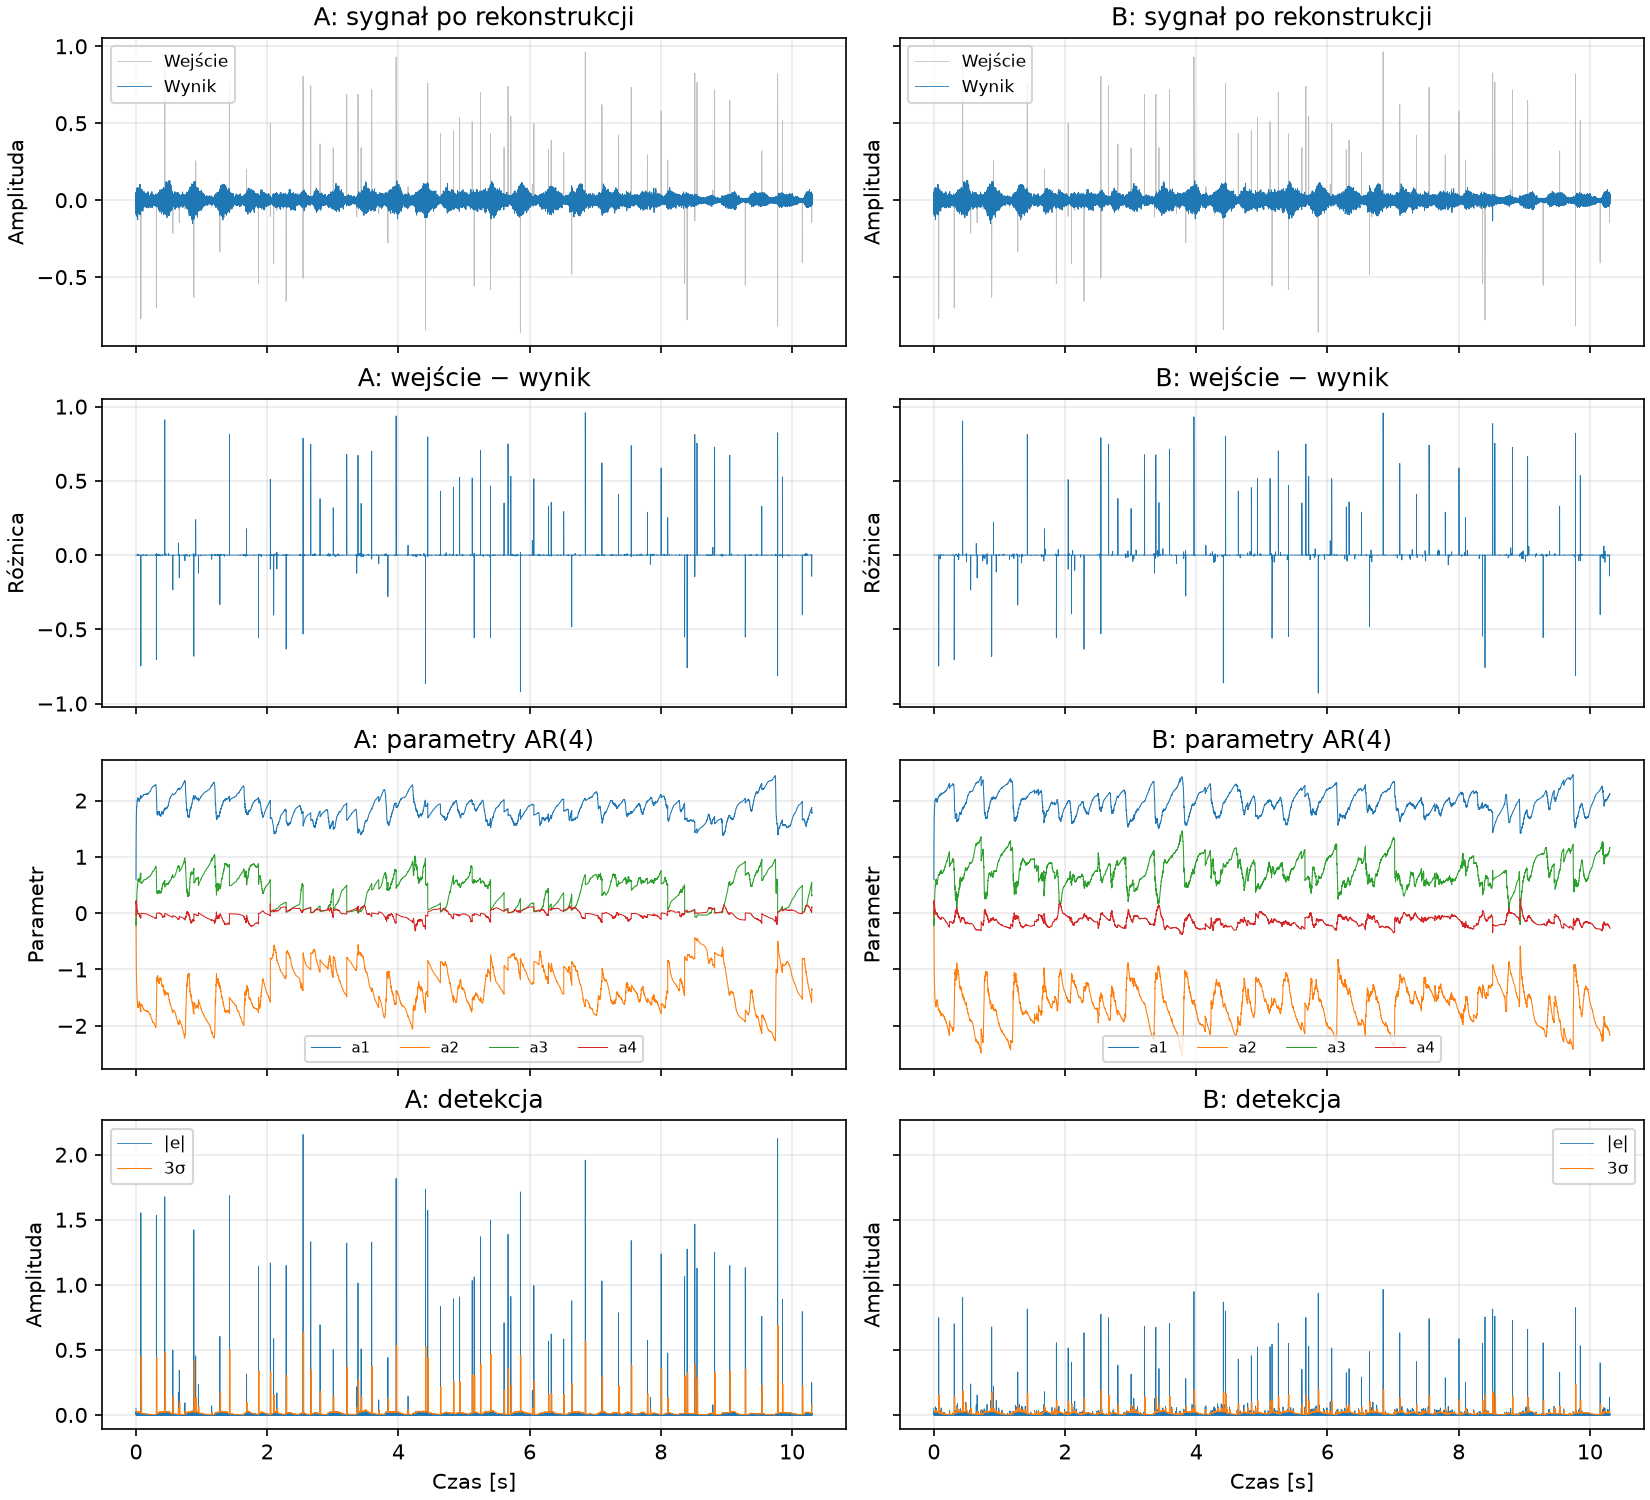
\includegraphics[width=\linewidth]{images/22_AB.png}
\caption{\texttt{22.wav}: A - z zakwestionowaną próbką, B - z ostatnią zaakceptowaną próbką.}
\end{figure}

\clearpage
\subsection{Nagranie 23.wav}
\begin{figure}[htbp]
\centering
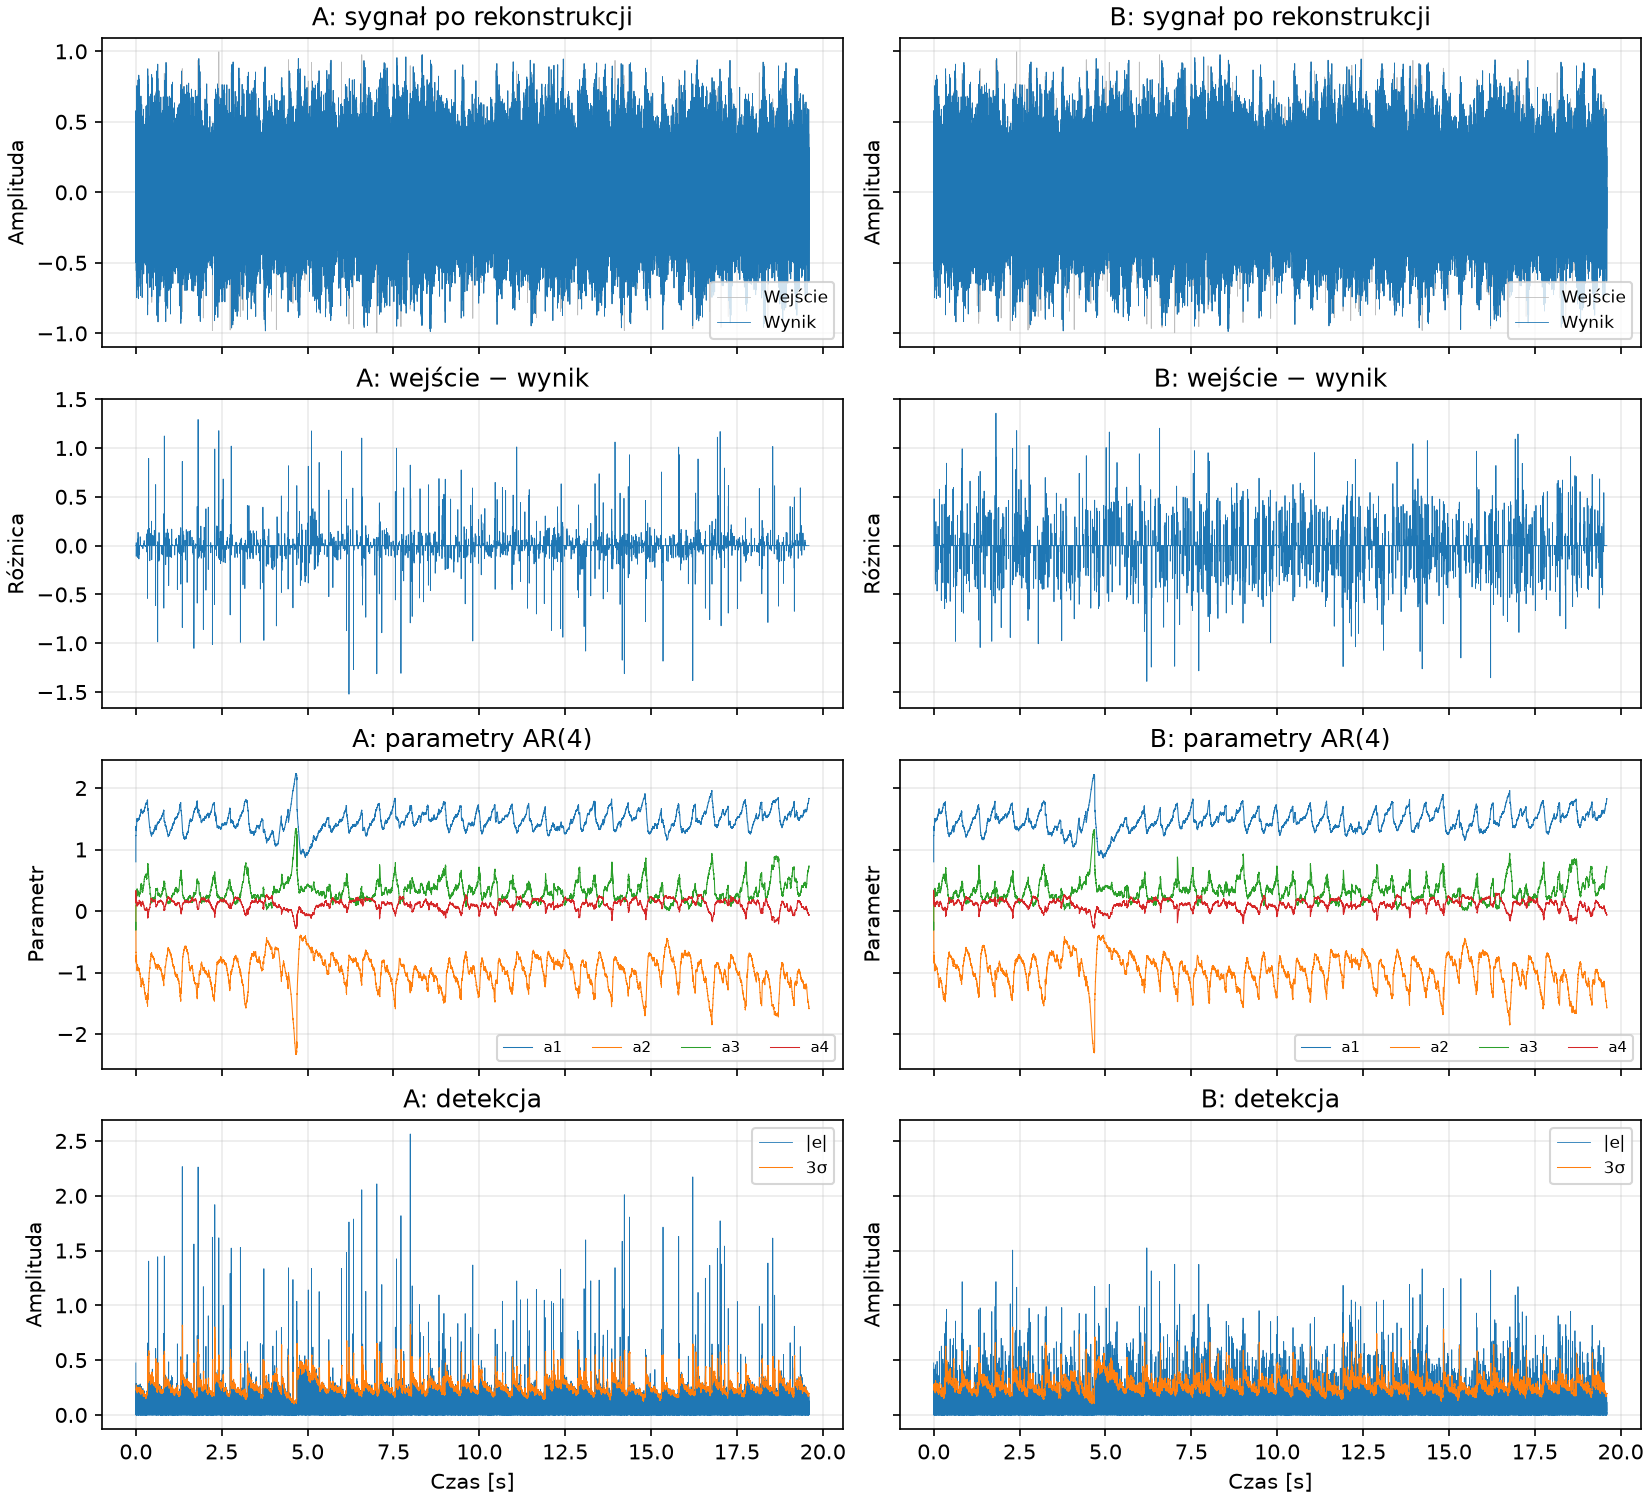
\includegraphics[width=\linewidth]{images/23_AB.png}
\caption{\texttt{23.wav}: A - z zakwestionowaną próbką, B - z ostatnią zaakceptowaną próbką.}
\end{figure}

\clearpage
\section{Wnioski}
B dał więcej detekcji i pominiętych serii we wszystkich nagraniach. W czterech naprawił mniej próbek niż A; wyjątek: \texttt{23.wav}.

A zachowuje zakłócenia w historii; B zastępuje je stałą wartością, co może wydłużać serie detekcji. Limit czterech detekcji może pomijać krótszy rzeczywisty trzask.

Statystyki nie rozstrzygają jakości. Pliki do odsłuchu: \texttt{NN\_A\_odszumiony.wav} oraz \texttt{NN\_B\_odszumiony.wav}.

\end{document}
